\documentclass{standalone}
\usepackage{standalone}

\begin{document}
  % 4. Software Architecture Diagram
  % 4.1 Context view
  % Describe the relationships, dependencies, and interactions between the
  % system and its environment (the people, system.. and external entities with
  % which it interacts). Your system in this view is represented by a blackbox
  % interacting with external entities. See example in Figure 1.
  % 4.2 Functional view
  % Describe the system’s runtime functional elements and their responsibility,
  % interfaces and primary int

  % Figure 1. Example of a context view

  % methodology:
  %   •	Represent each subcomponent of the system with a box in the figure. 
  %   •	Link the system subcomponents with connectors. These connectors define
  %     the interaction between the elements that use it. 
  %   •	Under the figure explain each subcomponent, and give:
  %   •	Inputs
  %   •	Outputs
  %   •	What functionality is available
  %   •	How to invoke each functionality (commands, syntax, …etc).
  \section{Architecture Diagrams}
  \begin{figure}[h]
    \caption{Context Diagram}
    \centering
    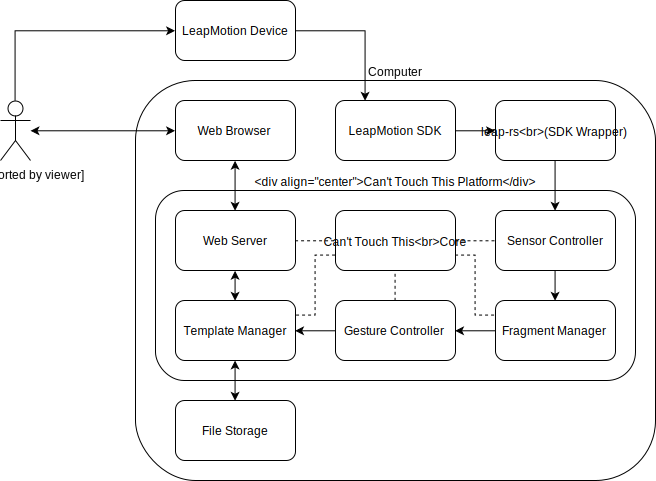
\includegraphics[width=\linewidth]{context-diagram}
  \end{figure}
  In this diagram, the \textit{Can't Touch This} platform displayed globally. It
  Shows three main objects:
  \begin{itemize}
    \tightlist{}
    \item The user
    \item The LeapMotion device
    \item The Can't Touch This platform
  \end{itemize}
  The user attaches the LeapMotion device to the computer, installs the platform
  and moves it's hand above the sensor to conduct an experiment. The LeapMotion
  device captures the data of the hand, and passes it on through the LeapMotion
  SDK, to the leap-rs wrapper. This leap-rs wrapper maps all functions made
  available through the LeapMotion SDK to the Rust programming language.
  Normally, a platform like \textit{Can't Touch This} would have to be
  programmed using the C programming language, as this is the language the SDK
  is written in.

  The leap-rs wrapper enables the SDK functionality in our platform, which we
  use in the Sensor Controller. The Sensor controller is our gateway of
  information, of our bits and bytes. The Sensor controller passes this data on
  to the Fragment Manager, which records all data and converts it into Points,
  Rotational Points (\textit{RotPoints}) and Traces of both kind. It even
  improves the recorded points in the trace by sampling them. Sampling is
  \ldots{}
  % TODO: Let Tim write this section

  After the conversion and sampling, the Gesture Controller receives the data
  and compares this to existing gestures, stored in the Template Manager. The
  Template Manager compares the received gesture to the existing ones stores on
  the system. The gestures are saved in text files, as the data is not that
  complex. If the system matches the current gestures with an existing one, it
  will give positive feedback through the web interface. The user will see the
  positive feedback and know that that gesture is working well.

  The web interface also retrieves all the stored gestures for the user to
  review. It can add and delete gestures as the user wants, except the
  pre-defined gestures.

  \begin{figure}[h]
    \caption{Context Diagram}
    \centering
    \includegraphics[width=\linewidth]{functional-diagram}
  \end{figure}
  \clearpage
\end{document}
